\begin{comment}
\begin{itemize}
  \item 6-2で,様々な顔の表示方法を提案した.
  \item コロナ禍の影響で十分な実験を行うことが出来なかった
  \item 提案したアプリケーションを用いて,十分な実験を行い,比較を行うことで,
  最適な表示方法を決定することが今後の課題である
  \item 一方で解決できていない問題も存在する
  \item 小窓が表示される際に,突然表示されて使用者が驚いてしまう
  \item 複数の人間に話しかけている場合の顔や小窓の表示方法
  \item 今後の研究でそれらの問題を解決する方法を模索していく
  \item また,今回のアプリケーションは個人対複数人といったユースケースに限られている
  \item 個人の参加者が複数人いた場合,OmniEyeBall上での表示をどのようにするかという問題がある.
  \item 例えば,OmniEyeBall側で,現在映したい人物を選択できるようにすれば,今回のシステムをそのまま活用できる
  \item 一方で,会話にPC使用者が複数人参加している場合には,同時に映すことが出来ない
  \item このようなユースケースにも対応していく方法も検討する必要がある
\end{itemize}
\end{comment}
本章では,5章で得られた知見に基づいていくつかのアプリケーションを
提案してきたが,以前解決できていない問題がある.

\subsubsection*{特定の一人を見ていないケース}
アンケート結果によって,小窓を既に表示されている顔の上に表示するのは
混乱を招いている可能性があると結論付けた.よって提案したアプリケーションでは
その表示方法を廃止した.しかし,先の表示方法は,実験用アプリケーションで特定の一人を見ていないケース
を区別していた表示方法であった.この状況を表す代替の表示方法を提示する必要がある.

案の一つとしては,テキストや印を表示する方法がある.
しかし,小さいとサインが見えにくく,大きすぎると
映像の邪魔になってしまう.なおかつ,本アプリケーションは
従来の方法に比べ,SUSの評価が向上したとは言えず,これ以上の
情報提示は,ただでさえ複雑なアプリケーションをさらに複雑にすると
考え,実装を見送った.

\subsubsection*{全天球ビデオカメラの回転の問題}

本アプリケーションは,使用開始前の
状態として,PCの使用者が全天球パノラマ画像の
中心部を見ている前提で,画像のスライドや顔認識した位置に
画像を張り付ける処理を行ってきた.しかし,カメラが回転すると,
基準としていた位置がずれ,ずらす処理にも変更を加える必要がある.
だが,本研究では回転を考慮した処理を行っていない.

これを解決する案として,特徴点マッチングを用いる方法が考えられる.
特徴点マッチングによって,画像のスライド距離を算出し,その値を
本論文の処理に加えて反映させれば,この問題は解決できるであろう.

\begin{figure}[tp]
  \centering
  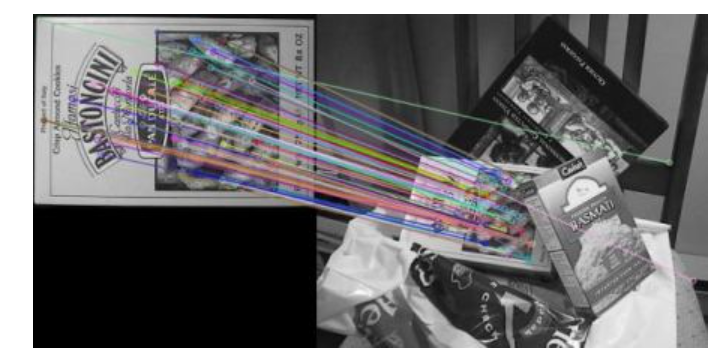
\includegraphics[scale=0.7]{fig/matching.png}
  \caption{特徴点マッチング} \cite{17}
\end{figure}

\subsubsection*{様々なケースへの対応}
今回は個人対複数人でのビデオ会議という状況
を前提において研究を進めてきた.しかし実際には
他にも以下のようなケースが存在する.
\begin{itemize}
  \item 複数のOmniEyeBallを使用するケース
  \item OmniEyeBallから孤立した参加者が複数人であるケース
  \item 孤立した参加者の何人かが共通の空間にいるケース
\end{itemize}

例えば2番目のケースは,OmniEyeBall側の参加者が現時点で注目したい
遠隔参加者を1人選ぶというようにする.さすれば,その1人に対して
今回提案したシステムが利用可能である.

しかし1番目のケース,3番目のケースは,複数人が同じ空間を
共有している.今回のような画像の回転を用いると,意図していない人物の
回転を同時に招いてしまう.これらの複雑なケースに沿ったシステムを
提案していくことは,今後の研究課題である.

\subsubsection*{まとめ}
今後の研究方針としては,先に述べたような
複雑なケースに対応するシステムの模索が考えられる.
一方,今回はコロナ禍の影響で,十分に実験が行えたとは言えない.
十分な時間を要して,今回提案した複数の表示方法について
綿密な実験を繰り返し,より多くのユーザーの実体験に
基づいた知見を獲得していくことも必要であろう.